%%%%%%%%%%%%%%%%%%%%%%%%%%%%%%%%%%%%%%%%%
% Beamer Presentation
% LaTeX Template
% Version 1.0 (10/11/12)
%
% This template has been downloaded from:
% http://www.LaTeXTemplates.com
%
% License:
% CC BY-NC-SA 3.0 (http://creativecommons.org/licenses/by-nc-sa/3.0/)
%
%%%%%%%%%%%%%%%%%%%%%%%%%%%%%%%%%%%%%%%%%

%----------------------------------------------------------------------------------------
%	PACKAGES AND THEMES
%----------------------------------------------------------------------------------------

\documentclass[10pt]{beamer}
\mode<presentation> {

% The Beamer class comes with a number of default slide themes
% which change the colors and layouts of slides. Below this is a list
% of all the themes, uncomment each in turn to see what they look like.

%\usetheme{default}
%\usetheme{AnnArbor}
%\usetheme{Antibes}
%\usetheme{Bergen}
%\usetheme{Berkeley}����JFIF����C
%\usetheme{Berlin}
%\usetheme{Boadilla}
%\usetheme{CambridgeUS}
%\usetheme{Copenhagen}
%\usetheme{Darmstadt}
%\usetheme{Dresden}
%\usetheme{Frankfurt}
%\usetheme{Goettingen}
%\usetheme{Hannover}
%\usetheme{Ilmenau}
%\usetheme{JuanLesPins}
%\usetheme{Luebeck}
%\usetheme{Madrid}
%\usetheme{Malmoe}
%\usetheme{Marburg}
%\usetheme{Montpellier}
\usetheme{PaloAlto}
%\usetheme{Pittsburgh}
%\usetheme{Rochester}
%\usetheme{Singapore}
%\usetheme{Szeged}
%\usetheme{Warsaw}

% As well as themes, the Beamer class has a number of color themes
% for any slide theme. Uncomment each of these in turn to see how it
% changes the colors of your current slide theme.

%\usecolortheme{albatross}
%\usecolortheme{beaver}
%\usecolortheme{beetle}
%\usecolortheme{crane}
%\usecolortheme{dolphin}
%\usecolortheme{dove}
%\usecolortheme{fly}
%\usecolortheme{lily}
%\usecolortheme{orchid}
%\usecolortheme{rose}
%\usecolortheme{seagull}
%\usecolortheme{seahorse}
\usecolortheme{whale}
%\usecolortheme{wolverine}

%\setbeamertemplate{footline} % To remove the footer line in all slides uncomment this line
\setbeamertemplate{footline}[page number] % To replace the footer line in all slides with a simple slide count uncomment this line

%\setbeamertemplate{navigation symbols}{} % To remove the navigation symbols from the bottom of all slides uncomment this line
}

\usepackage{graphicx} % Allows including images
\usepackage{booktabs} % Allows the use of \toprule, \midrule and \bottomrule in tables
\usepackage{amsmath}
\usepackage{subfig}
\usepackage{caption}
\usepackage{mathabx}
\usepackage{wasysym}
\usepackage{wrapfig}
\usepackage{tikz}
\usepackage{animate}
\usepackage{minted}
\usepackage{listings}
\usepackage{listings}
\usetikzlibrary{shapes.geometric, arrows}
\usepackage{minted}
\usepackage{color}

\usepackage{xcolor}
\usepackage{listings}
\lstset{basicstyle=\ttfamily,
  showstringspaces=false,
  commentstyle=\color{red},
  keywordstyle=\color{blue}
}

%\usepackage{subcaption}
%----------------------------------------------------------------------------------------
%	TITLE PAGE
%----------------------------------------------------------------------------------------
\title[]{Lab \#3: Software Defined Radio \\ RDS signal analysis } % The short title appears at the bottom of every slide, the full title is only on the title page

\author{Alexander Blaauwgeers \\ \& \\ Bernardus Jansen} % Your name
\institute[University of Amsterdam] % Your institution as it will appear on the bottom of every slide, may be shorthand to save space
{
University of Amsterdam \\ % Your institution for the title page
\medskip
%\textit{john@smith.com} % Your email address
}
\date{April 20, 2018} % Date, can be changed to a custom date

\begin{document}

\begin{frame}
\titlepage % Print the title page as the first slide
\end{frame}

%----------------------------------------------------------------------------------
\section{Introduction }
\begin{frame}{Introduction}
\begin{block}{Question}
There are radio stations that send out RDS information so you know traffic jams are ahead or know the name of the
song that is currently playing.
\begin{itemize}
    \item Is there a way to retrieve this information using SDR?
    \item What kind of information can you get out of this?
    \item How does the protocol work?
\end{itemize}
\end{block}
\end{frame}

\begin{frame}{What is RDS?}
Radio Data System

\begin{itemize}
    \item Allows to send data over FM radio
    \item Multiple fields
    \begin{itemize}
        \item Most only flags or short identifiers
    \end{itemize}
    \item Radio Text field
    \begin{itemize}
        \item Allows for arbitrary 64-character strings
    \end{itemize}
    \item Traffic Message Channel
    \begin{itemize}
        \item Often encoded
    \end{itemize}
\end{itemize}
\end{frame}

%----------------------------------------------------------------------------------
\section{Theory}
%----------------------------------------------------------------------------------
\begin{frame}{Theory}
\centering
\begin{itemize}
    \item Data is carried on a 57kHz subcarrier
\end{itemize}

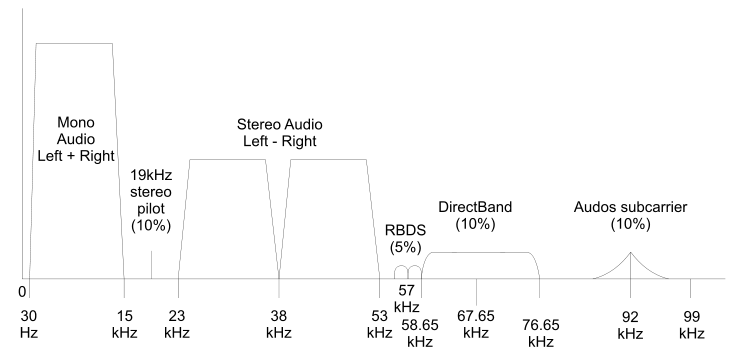
\includegraphics[width=\textwidth]{fmspectrum.png}

\end{frame}

%----------------------------------------------------------------------------------
\section{Receiving RDS}
\begin{frame}[fragile]{Receiving RDS Signals}
\begin{itemize}
    \item GQRX allows to receive RDS channel information natively
    \begin{itemize}
        \item But only basic and interpreted information
    \end{itemize}
    \item \verb|redsea|
    \begin{itemize}
        \item Low level tool that can extract all raw RDS fields from \verb|rtl_fm| input
    \end{itemize}
\end{itemize}
\end{frame}

%----------------------------------------------------------------------------------
\section{Transmitting RDS}

\begin{frame}{Security}
    \pause \centering None
\end{frame}

\begin{frame}{Transmitting RDS Signals}

\begin{itemize}
    \item It is possible to send FM/RDS signals with your own transmitter
    \begin{itemize}
        \item Possible to make users switch channels with the appropriate flags
        \item Display arbitrary text on user radio displays
        \pause \item But it is illegal (exept below 50 nW) \footnote{\tiny{Subcategorie 8.C "Regeling gebruik van frequentieruimte zonder vergunning en zonder meldingsplicht 2015"}}
    \end{itemize}
\end{itemize}



\end{frame}

%----------------------------------------------------------------------------------
\section{PoC - 102.3 MHz}
\begin{frame}{Hardware}
    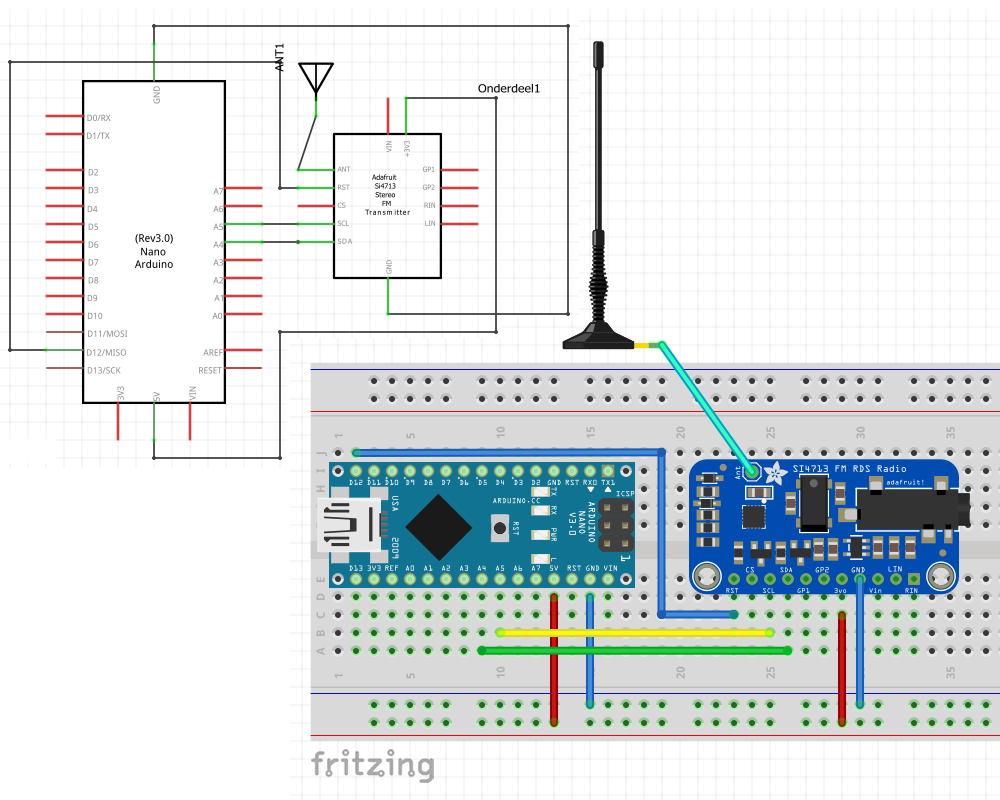
\includegraphics[width=9cm]{FMzend.png}
\end{frame}

\begin{frame}{Code}
    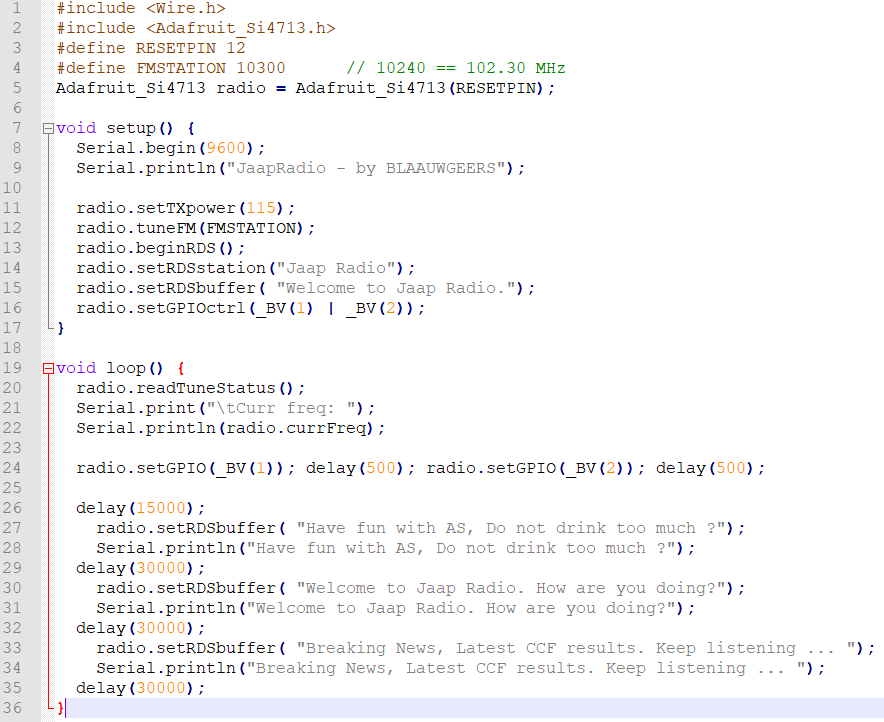
\includegraphics[width=9cm]{FMcode.png}
\end{frame}

\begin{frame}{102.3 MHz}
    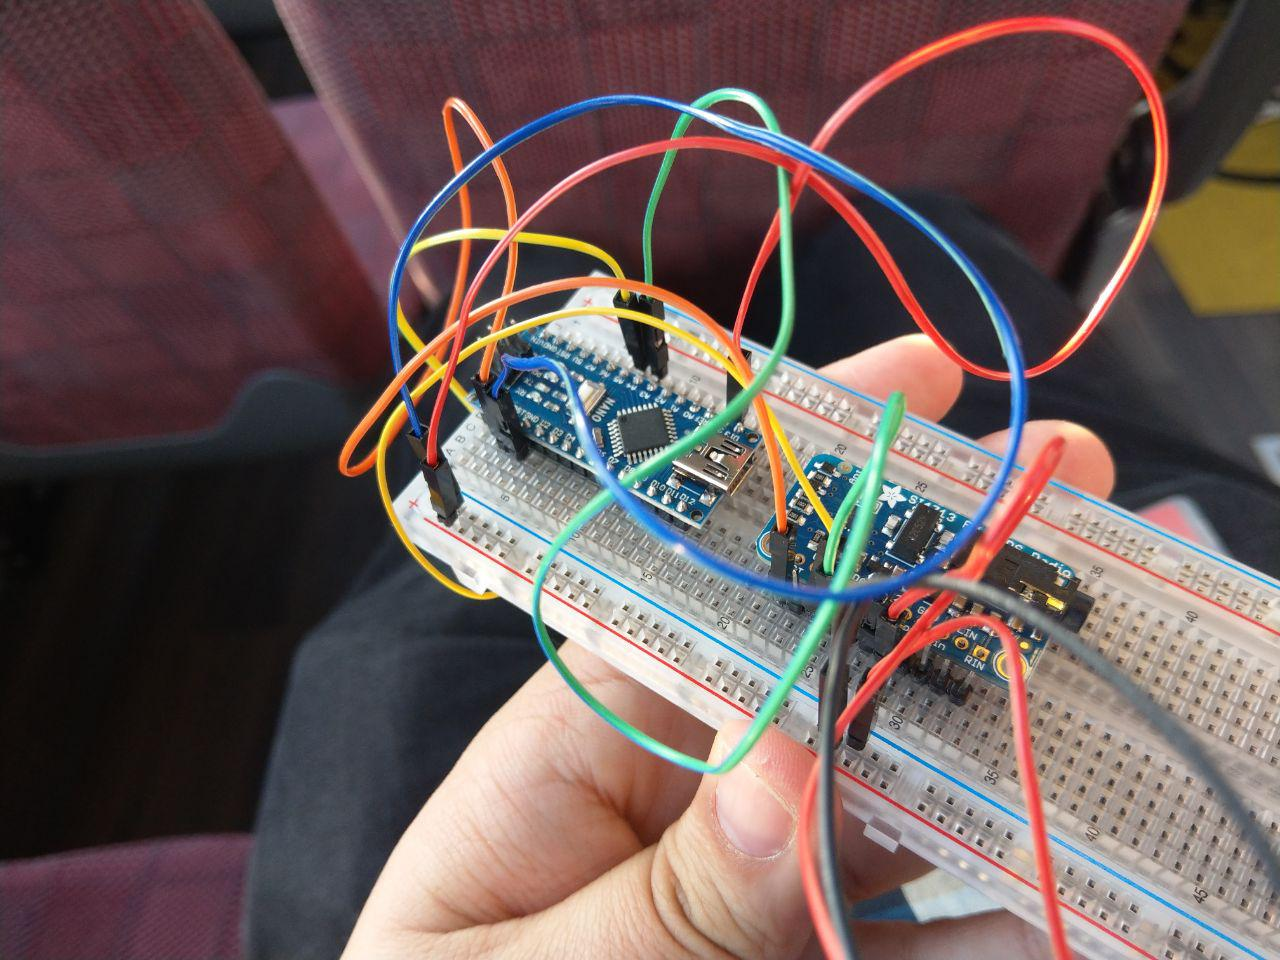
\includegraphics[width=9cm]{photo_2018-04-20_10-12-16.jpg}
\end{frame}

%----------------------------------------------------------------------------------

%----------------------------------------------------------------------------------

\begin{frame}{Questions?}

Questions?

%\def\newblock{}
%\bibliographystyle{unsrt}
%\bibliography{mybib}
\end{frame}

\end{document} 
%---------------------------------------------------------------------------
